\documentclass[10pt,twocolumn,letterpaper]{article}

\usepackage[margin=0.75in]{geometry}
\usepackage{amsmath,amssymb,amsfonts}
\usepackage{graphicx}
\usepackage{booktabs}
\usepackage{tabularx}
\usepackage{multirow}
\usepackage{hyperref}
\usepackage{cite}
\usepackage{enumitem}
\usepackage{tikz}
\usetikzlibrary{shapes.geometric,arrows.meta,positioning,calc}
\usepackage{listings}
\usepackage{xcolor}
\usepackage{titlesec}

\hypersetup{
    colorlinks=true,
    linkcolor=blue!70!black,
    citecolor=blue!70!black,
    urlcolor=blue!70!black
}

\titleformat{\section}{\large\bfseries}{\thesection.}{0.5em}{}
\titleformat{\subsection}{\normalsize\bfseries}{\thesubsection}{0.5em}{}
\titleformat{\subsubsection}{\small\bfseries}{\thesubsubsection}{0.5em}{}

\title{\textbf{Cloudra: An Autonomous Multi-Agent Research Runtime for Quantum-Chemical Organic Reaction Mechanism Elucidation}}

\author{
    Cloudra Team \\
    \small Changsha University of Science and Technology, Changsha, China \\
    \small Correspondence: \texttt{951899550@qq.com}
}
\date{}

\begin{document}

\maketitle

\begin{abstract}
Determining reaction mechanisms in homogeneous organic chemistry demands intricate multi-step quantum-chemical workflows, including conformational sampling, transition state (TS) searches, intrinsic reaction coordinate (IRC) tracking, and solution-phase thermochemistry. While large language model (LLM) agents have demonstrated promise across scientific domains, existing computational chemistry agents either focus on heterogeneous catalytic surfaces or execute disconnected quantum-chemical scripts without validating endpoint connectivity or free-energy profiles. Furthermore, current autonomous agents frequently suffer from ``completion by assertion,'' where an agent self-declares success without rigorous verification. Here we report \textbf{Cloudra}, an autonomous multi-agent system designed for end-to-end quantum-chemical elucidation of homogeneous organic reaction mechanisms from reactant and product specifications. Cloudra establishes a \textbf{Delivery Directed Acyclic Graph (Delivery DAG)} orchestration architecture, transforming mechanistic elucidation into a deterministically audited contract. Each elementary step is governed by an ordered stage contract (TS guess, saddle optimization, frequency verification, bidirectional IRC, endpoint optimization, and quasi-harmonic thermochemistry) where stage progression requires reproducible computational evidence. Cloudra additionally incorporates a domain-specialized \textbf{Computational Chemistry Knowledge Graph (GraphRAG)} that distills domain methodology and troubleshooting heuristics into evidence-tiered, falsification-aware causal decision trees---an updatable scientific memory layer that complements the frozen parametric knowledge of pre-trained models. To eliminate coordinate hallucinations, Cloudra enforces structural guards preventing direct manipulation of atomic coordinates. Orchestrated by an asynchronous, peer-to-peer event-driven runtime, Cloudra coordinates specialized sub-agents with electronic-structure perception for open-shell radical centers and hydrogen-bonding networks. Cloudra is systematically evaluated on a curated 100-reaction benchmark spanning four difficulty tiers (Easy, Normal, Hard, and Impossible with justified refusal) through a two-stage serial ablation, establishing that supervisory DAG gating eliminates completion hallucinations ($0.0\%$) while Knowledge Graph augmentation substantially accelerates error recovery and reduces wasted compute. Finally, the fully integrated system achieves a practical closed loop across three demanding real-world research problems: a hexafluoroisopropanol (HFIP)-mediated hydrogen-bonding cluster pathway solved via human-agent collaboration, a stereoselective axial-chiral transformation with quantitative $ee$ prediction, and an open-shell small-molecule radical reaction under complex electronic states. Across these benchmarks and applications, Cloudra autonomously generates competing mechanistic hypotheses, navigates potential energy surfaces, and delivers verifiable mechanistic networks, establishing a rigorous paradigm for autonomous discovery in molecular quantum chemistry.
\end{abstract}

\section{Introduction}
Elucidating reaction mechanisms is fundamental to understanding and designing organic chemical transformations \cite{fukui1981irc}. In contemporary computational organic chemistry, resolving a reaction mechanism requires constructing an unbroken chain of quantum-chemical evidence. Starting strictly from reactant and product molecular graphs, a computational chemist must identify atom mappings, perform conformational ensemble searches across flexible intermediates \cite{grimme2019crest}, generate viable transition state (TS) guesses \cite{smidstrup2014idpp}, optimize first-order saddle points, confirm exactly one imaginary vibrational frequency, track bidirectional intrinsic reaction coordinates (IRC) to connected minima, optimize those endpoints, verify product identity, and compute solution-phase thermochemical corrections \cite{grimme2012goodvibes}. For complex homogeneous transformations involving open-shell radical intermediates, non-covalent solvent clusters (e.g., hexafluoroisopropanol, HFIP), or atropisomeric axial chirality, navigating this multi-dimensional potential energy surface (PES) remains an intensive manual endeavor.

Recent advances in large language models (LLMs) and autonomous agentic systems have sparked significant interest in automating scientific workflows \cite{boiko2023autonomous,bran2024chemcrow,swanson2025virtuallab,coscientist2026}. In chemistry, multi-agent frameworks have automated wet-lab synthesis planning \cite{boiko2023autonomous}, tool-augmented property estimation \cite{bran2024chemcrow}, and open-source robotic execution \cite{song2025chemagents}. In computational chemistry, systems such as El Agente \cite{zou2025elagente} and ChemGraph \cite{chemgraph2026} have automated script generation and thermodynamics workflows, while automated reaction-profile tools such as autodE \cite{young2021autode} and the Artificial Force Induced Reaction (AFIR) method \cite{sameera2016afir} have long automated transition-state assembly from elementary reaction topologies. Closer to autonomous mechanism discovery, ARplorer \cite{arplorer2025} demonstrated LLM-guided automated reaction path exploration for quantum-chemical minimum energy paths, whereas TSAgent \cite{tsagent2026} performed autonomous transition state searching on heterogeneous catalytic surfaces using nudged elastic band (NEB) calculations, CatDT \cite{catdt2026} explored digital twin verification for heterogeneous catalysis networks, and AdsMind \cite{adsmind2026} established physical feedback loops for automated surface adsorption discovery. Beyond surface chemistry, the broader autonomous-science landscape spans tool-augmented scientific reasoning \cite{ma2024sciagent}, quantum-computing experiment automation \cite{cao2025agents}, and physics-aware multi-agent materials research \cite{ghafarollahi2024atomatoms}.

Despite these advancements, autonomous mechanistic elucidation for \textbf{homogeneous organic small-molecule chemistry} remains completely unaddressed: none of the systems above delivers end-to-end mechanism elucidation with verified endpoint connectivity and complete free-energy profiles. As highlighted in recent critical evaluations of autonomous scientific agents \cite{canai2026,yik2024chatgpt} and large-scale chemical-reasoning benchmarks \cite{mirza2025chembench}, current architectures face three fundamental limitations:
\begin{enumerate}[leftmargin=*]
\item \textbf{Chemical Domain and Methodological Disconnect:} Existing transition state agents (e.g., TSAgent \cite{tsagent2026}) are tailored for periodic surface catalysis using plane-wave density functional theory (DFT) and NEB. Homogeneous organic chemistry operates on localized molecular wavefunctions where reaction paths involve delicate conformational pre-organization, concerted bond reorganization, open-shell radical spin states ($\langle S^2 \rangle$ contamination), and explicit solvent-solute hydrogen-bonding clusters. Point-and-click workflow executors (such as Aitomia \cite{aitomia2026}) execute user-requested individual tasks at semi-empirical levels without autonomous hypothesis generation, atom mapping, or endpoint verification.
\item \textbf{The ``Completion by Assertion'' Fallacy:} In typical LLM-agent implementations, task completion is determined by the agent's internal prose generation. When an agent encounters an SCF convergence failure or a stationary point with spurious imaginary frequencies, it often asserts in text that the mechanism is resolved, fabricating conclusions without physical evidence \cite{yik2024chatgpt,canai2026}.
\item \textbf{Fragile Coordinate Hallucination:} Standard LLMs frequently hallucinate or corrupt Cartesian coordinate blocks when passing intermediate 3D structures between steps, breaking numerical continuity across quantum chemistry codes.
\end{enumerate}

To overcome these foundational challenges, we present \textbf{Cloudra}, an autonomous multi-agent research runtime engineered specifically for homogeneous organic reaction mechanism elucidation. Cloudra introduces five core innovations:
\begin{itemize}[leftmargin=*]
\item \textbf{Homogeneous Organic Mechanism Elucidation as the Target Domain:} Unlike surface-catalysis agents (TSAgent, CatDT, AdsMind) or script-level workflow executors (El Agente, ChemGraph, Aitomia), Cloudra targets end-to-end elucidation of homogeneous organic small-molecule mechanisms---from reactant and product graphs to competing, fully verified mechanistic networks with complete free-energy profiles.
\item \textbf{Evidence-Delivered DAG Architecture \& Ordered Stage Contracts:} We formalize reaction mechanism elucidation as a Delivery Directed Acyclic Graph (Delivery DAG). Mechanistic completion is governed by an immutable evidence ledger and deterministic stage contracts ($s_1 \rightarrow s_8$), replacing conversational assertions with verifiable computational proofs.
\item \textbf{Chemistry-Native Tool Suite as Scientific Instruments:} Beyond guarding against hallucination, Cloudra's chemistry-native tools convert domain expertise into instrument-grade, reproducible measurements: \texttt{ts\_guess} strict verification proves path-direction consistency with a single imaginary frequency and bidirectional IRC endpoints; electronic-structure perception (IBO localization, Mayer bond orders, meta-L\"owdin spin densities) reads bond-forming and bond-breaking events and open-shell spin states programmatically; \texttt{internal\_coordinates} flags compressed, elongated, breaking, and forming bonds with hybridization anomalies; and all Cartesian transformations are routed through verified backends under strict \texttt{coord\_guard} policies.
\item \textbf{Computational Chemistry Knowledge Graph (GraphRAG) as Structured Scientific Memory:} Cloudra integrates a domain-specialized knowledge graph of methodology and troubleshooting heuristics (e.g., saddle point multi-imaginary frequency elimination, SCF oscillation damping, spin-contamination mitigation, explicit solvent cluster selection, and multireference diagnostics) into \textbf{evidence-tiered, falsification-aware causal decision trees}, providing an updatable scientific memory orthogonal to frozen model weights and flat episode libraries.
\item \textbf{Peer-to-Peer Asynchronous Multi-Agent Runtime:} Built on an event-sourced runtime (Runtime v2), Cloudra orchestrates specialized sub-agents communicating through an open peer-to-peer forum (\texttt{AgentHub}) and supervised by an independent scientific audit agent (\texttt{Supervisor}).
\end{itemize}

To evaluate Cloudra rigorously, we pursue a systematic two-stage validation strategy. First, we design a \textbf{100-reaction benchmark test set} categorized into four distinct difficulty tiers (Easy, Normal, Hard, and Impossible with justified refusal) and perform a \textbf{two-stage serial ablation}: (i) evaluating DAG orchestration modes (\texttt{standard} vs. \texttt{dag\_record} vs. \texttt{dag\_guided}) to demonstrate that supervisory DAG gating deterministically enforces scientific rigor and eliminates completion hallucinations ($0.0\%$), and (ii) evaluating the addition of the computational chemistry Knowledge Graph (\texttt{dag\_guided} vs. \texttt{dag\_guided + GraphRAG}) to show that structured decision support significantly accelerates error recovery and reduces wasted compute. Second, having validated the individual and integrated components on the benchmark, we deploy the final, fully-equipped Cloudra system onto \textbf{three demanding real-world research problems}---an HFIP solvent-cluster mediated quinone synthesis via human-agent collaboration, an axially chiral atropisomeric transformation with quantitative enantioselectivity prediction, and an open-shell small-molecule radical reaction under complex electronic states---establishing a practical closed loop from synthetic benchmarking to frontline computational organic chemistry.

\section{System Architecture and Methodology}

Cloudra is organized as an anarchic peer collective rather than a hierarchical agent tree: all agents share equal standing and differ only in their division of labor. Four pillars uphold this design (Figure~\ref{fig:architecture}): (1) \texttt{AgentHub}, the peer-to-peer collaboration fabric connecting all agents directly; (2) an event-sourced research runtime (Runtime v2) beneath the collective; (3) a Delivery Directed Acyclic Graph (Delivery DAG) evidence engine with deterministic gating, watched over by an independent Supervisor that serves as the gatekeeper of delivery; and (4) a domain-specialized Computational Chemistry Knowledge Graph (\texttt{GraphRAG}) layer providing structured diagnostic decision trees and cross-task troubleshooting heuristics.

\begin{figure*}[t]
\centering
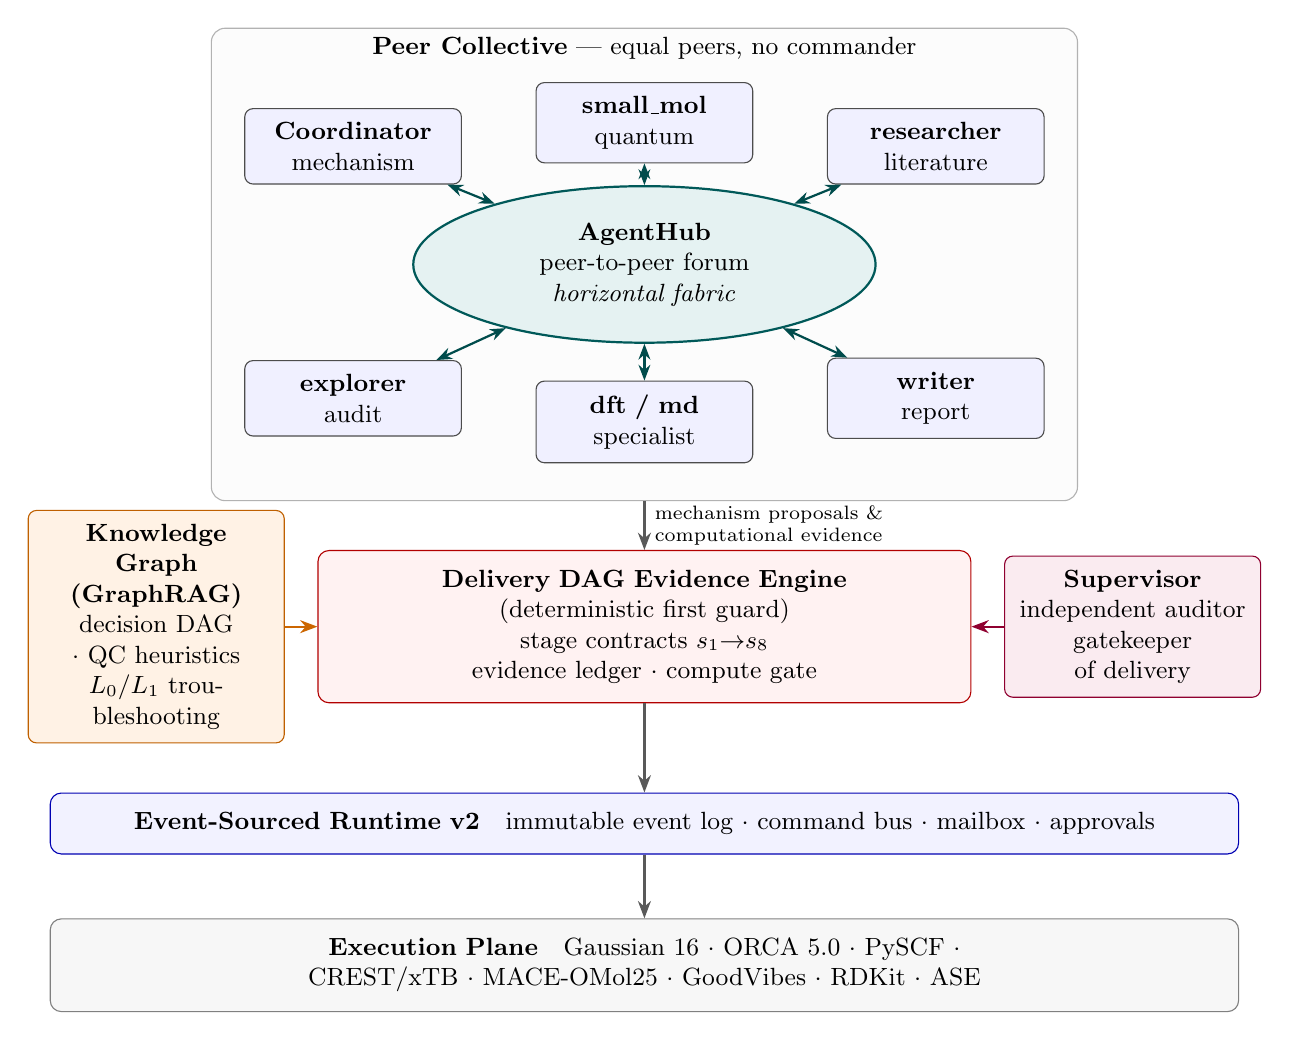
\begin{tikzpicture}[
    font=\small,
    agent/.style={rectangle, draw=black!70, fill=blue!6, rounded corners=3pt, inner sep=5pt, text width=2.4cm, align=center},
    hub/.style={ellipse, draw=teal!70!black, fill=teal!10, thick, inner sep=5pt, text width=3.8cm, align=center},
    sup/.style={rectangle, draw=purple!75!black, fill=purple!8, rounded corners=3pt, inner sep=5pt, text width=2.9cm, align=center},
    kg/.style={rectangle, draw=orange!75!black, fill=orange!10, rounded corners=3pt, inner sep=5pt, text width=2.9cm, align=center},
    band/.style={rectangle, draw=black!30, rounded corners=5pt, fill=gray!2, inner sep=12pt},
    plane/.style={rectangle, rounded corners=4pt, inner sep=7pt, align=center},
    dagplane/.style={plane, draw=red!70!black, fill=red!5, text width=7.8cm},
    rtplane/.style={plane, draw=blue!70!black, fill=blue!5, text width=14.6cm},
    exeplane/.style={plane, draw=black!50, fill=black!3, text width=14.6cm},
    link/.style={{Stealth[length=2mm]}-{Stealth[length=2mm]}, thick, draw=teal!60!black},
    arrow/.style={-{Stealth[length=2.2mm]}, thick, draw=black!65}
]

% --- Band 1: peer collective (equal agents around the hub) ---
\node[band, minimum width=11.0cm, minimum height=6.0cm] (peer) at (0,3.2) {};
\node[hub] (hub) at (0,3.2) {\textbf{AgentHub}\\peer-to-peer forum\\\textit{horizontal fabric}};
\node[agent] (coord) at (-3.7,4.7) {\textbf{Coordinator}\\mechanism};
\node[agent] (smallmol) at (0,5.0) {\textbf{small\_mol}\\quantum};
\node[agent] (researcher) at (3.7,4.7) {\textbf{researcher}\\literature};
\node[agent] (explorer) at (-3.7,1.5) {\textbf{explorer}\\audit};
\node[agent] (dftmd) at (0,1.2) {\textbf{dft / md}\\specialist};
\node[agent] (writer) at (3.7,1.5) {\textbf{writer}\\report};
\draw[link] (hub) -- (coord);
\draw[link] (hub) -- (smallmol);
\draw[link] (hub) -- (researcher);
\draw[link] (hub) -- (explorer);
\draw[link] (hub) -- (dftmd);
\draw[link] (hub) -- (writer);
\node[anchor=north] (peerlabel) at (peer.north) {\textbf{Peer Collective} --- equal peers, no commander};

% --- Band 2: governance & knowledge (flanking the Delivery DAG) ---
\node[dagplane] (dagp) at (0,-1.4) {\textbf{Delivery DAG Evidence Engine}\\(deterministic first guard)\\stage contracts $s_1{\rightarrow}s_8$\\evidence ledger $\cdot$ compute gate};
\node[kg] (kgnode) at (-6.2,-1.4) {\textbf{Knowledge Graph (GraphRAG)}\\decision DAG $\cdot$ QC heuristics\\$L_0/L_1$ troubleshooting};
\node[sup] (sup) at (6.2,-1.4) {\textbf{Supervisor}\\independent auditor\\gatekeeper of delivery};
\draw[arrow, draw=orange!80!black] (kgnode.east) -- (dagp.west);
\draw[arrow, draw=purple!75!black] (sup.west) -- (dagp.east);

% --- Band 3 & 4: runtime and execution ---
\node[rtplane] (rtp) at (0,-3.9) {\textbf{Event-Sourced Runtime v2}\quad immutable event log $\cdot$ command bus $\cdot$ mailbox $\cdot$ approvals};
\node[exeplane] (exep) at (0,-5.7) {\textbf{Execution Plane}\quad Gaussian 16 $\cdot$ ORCA 5.0 $\cdot$ PySCF $\cdot$ CREST/xTB $\cdot$ MACE-OMol25 $\cdot$ GoodVibes $\cdot$ RDKit $\cdot$ ASE};

\draw[arrow] (peer.south) -- (dagp.north) node[midway, right, font=\scriptsize, align=left] {mechanism proposals \&\\computational evidence};
\draw[arrow] (dagp.south) -- (rtp.north);
\draw[arrow] (rtp.south) -- (exep.north);

\end{tikzpicture}
\caption{\textbf{Cloudra peer-collective architecture.} All agents are peers of equal standing with complementary divisions of labor; no agent commands another. \texttt{AgentHub} is the connective fabric of the system, enabling direct horizontal peer-to-peer communication. The \textbf{Knowledge Graph (GraphRAG)} layer provides domain-specialized diagnostic decision trees for real-time quantum-chemical troubleshooting. The \textbf{Supervisor} is independent of the agent collective and serves as the gatekeeper of the Delivery DAG---a second, scientific guard on top of deterministic evidence verification.}
\label{fig:architecture}
\end{figure*}

\subsection{Event-Driven Runtime and Agent Roles}
Unlike conventional synchronous conversational loops, Cloudra operates on an asynchronous event-driven core (\texttt{Runtime v2}). State transitions, tool invocations, and agent dialogues are logged as immutable events within an event log. This design ensures that every computational conclusion is fully reproducible and replayable across interrupted execution runs.

Cloudra organizes research workflows through specialized agent roles rather than a single monolithic LLM prompt:
\begin{itemize}[leftmargin=*]
\item \textbf{Coordinator:} The mechanism architect role---a peer among equals, not a superior of other agents. It decomposes overall objectives, proposes reaction networks, designs stage contracts, and synthesizes intermediate findings; coordination itself emerges through \texttt{AgentHub} rather than through centralized command.
\item \textbf{small\_mol (Quantum Chemist):} Specializes in molecular quantum mechanics, orchestrating conformer generation, coordinate scans, transition state optimizations, vibrational analyses, and electronic structure diagnostics.
\item \textbf{researcher (Literature Specialist):} Queries bibliographic databases (OpenAlex, arXiv) to extract reported reaction conditions, analogous mechanisms, and kinetic parameters.
\item \textbf{explorer (Code \& Workspace Auditor):} Performs read-only inspection of trajectory logs, output files, and data structures.
\item \textbf{Supervisor (Scientific Auditor):} A dedicated evaluation agent operating under \texttt{dag\_guided} mode. The Supervisor independently audits proposed mechanism drafts, reviews incoming computational evidence from \texttt{CallReview} queues, and enforces adherence to peer-review quantum-chemical standards.
\end{itemize}

\subsection{Peer-to-Peer Collaboration via AgentHub}
To avoid communication bottlenecks inherent in strictly centralized hierarchical agent trees, Cloudra features \textbf{AgentHub}, an open peer-to-peer forum that functions as the glue of the system. Every agent---including the Coordinator---communicates through AgentHub directly: parallel sub-agents broadcast reusable computational findings (such as discovered low-energy conformers, optimized basis set parameters, or spin-contamination warnings), pose cross-domain queries, and conduct direct peer calls. Because all shared knowledge is posted as addressable, threaded artifacts, AgentHub's post/topic structure enables seamless real-time horizontal information exchange.

When a specialized agent identifies an electronic structure anomaly (e.g., severe spin contamination $\langle S^2 \rangle > 0.85$ on a nominally doublet intermediate), it posts a finding to AgentHub, enabling parallel workers to immediately adapt their functional or basis set configurations without waiting for global round-trip orchestration.

\subsection{Delivery DAG Formalism and Ordered Stage Contracts}
The defining formal mechanism in Cloudra is the \textbf{Delivery Directed Acyclic Graph (Delivery DAG)}. In Cloudra, a proposed reaction mechanism is represented as a typed directed graph $\mathcal{G} = (\mathcal{V}, \mathcal{E})$:
\begin{itemize}[leftmargin=*]
\item \textbf{Occurrence Nodes ($v \in \mathcal{V}$):} Represent distinct chemical species (reactants, intermediates, products, and non-covalent solvent complexes) assigned with canonical SMILES representations and formal roles.
\item \textbf{Elementary Step Edges ($e \in \mathcal{E}$):} Represent elementary chemical transformations connecting source and target species nodes.
\end{itemize}

Crucially, Cloudra eliminates ``completion by assertion'' by binding every graph element to an immutable \textbf{Stage Contract}. An elementary step edge $e_{ij}$ is required to pass through a strictly ordered sequence of physical verification stages:
\begin{equation}
\text{Stage Sequence: } s_1 \rightarrow s_2 \rightarrow s_3 \rightarrow s_4 \rightarrow s_5 \rightarrow s_6 \rightarrow s_7 \rightarrow s_8
\end{equation}
Where:
\begin{enumerate}[leftmargin=*]
\item $s_1 = \texttt{ts\_guess}$: Preliminary transition state geometric hypothesis generated via IDPP interpolation or relaxed coordinate scan (advisory).
\item $s_2 = \texttt{ts\_opt}$: First-order saddle point optimization convergence under quantum-chemical electronic structure methods (e.g., DFT / MLIP).
\item $s_3 = \texttt{frequency}$: Harmonic vibrational analysis verifying exactly one imaginary vibrational frequency ($n_\mathrm{imag} = 1$) corresponding to the target reaction vector.
\item $s_4 = \texttt{short\_irc}$: Initial bidirectional steepest-descent displacement along the transition vector ($\Delta s > 0$ and $\Delta s < 0$) confirming exit from the saddle region.
\item $s_5 = \texttt{endpoint\_a}$: Full gradient relaxation of the forward trajectory to a stationary intermediate, confirming connectivity to target species $v_j$.
\item $s_6 = \texttt{endpoint\_b}$: Full gradient relaxation of the backward trajectory, confirming connectivity to source species $v_i$.
\item $s_7 = \texttt{direction}$: Verification of geometric and reaction coordinate orientation consistency between endpoints and the transition state.
\item $s_8 = \texttt{thermochemistry}$: Quasi-harmonic free energy evaluation (including solvent corrections and low-frequency entropy damping) at standard state.
\end{enumerate}

A stage $s_k$ cannot be bound until all antecedent required stages $s_{1 \dots k-1}$ are either fully supported by parsed computational artifacts or explicitly waived with scientific justification.

\subsection{Deterministic Gating, coord\_guard, and Three-Mode Ablation}
To guarantee that neither LLM hallucinations nor unverified claims bypass scientific verification, Cloudra embeds deterministic runtime policies directly into the tool-execution pipeline:
\begin{enumerate}[leftmargin=*]
\item \textbf{Substantive Compute Gating:} When a mechanism is initialized, the Coordinator must formulate a formal hypothesis via \texttt{dag\_propose\_mechanism}. Direct computational submission tools (\texttt{submit\_compute\_job}, \texttt{gjf\_writer}) remain locked until the hypothesis graph and stage contracts are accepted by the Supervisor (or auto-accepted under record mode), preventing unguided resource exhaustion.
\item \textbf{coord\_guard (Coordinate Hallucination Firewall):} LLMs exhibit notorious difficulty in outputting accurate floating-point Cartesian atomic matrices. Attempting to write hand-crafted coordinate matrices directly into \texttt{.gjf} or \texttt{.xyz} files triggers runtime policy warnings. All 3D structural operations must originate from verified structural generation tools (\texttt{smiles\_to\_mol}, \texttt{conformer\_search}, \texttt{internal\_coordinates}, \texttt{ts\_guess}).
\item \textbf{Electronic Structure Perception:} Open-shell and radical systems require vigilant monitoring of non-physical spin states. Cloudra provides native electronic analysis tools extracting Mulliken and meta-Löwdin atomic spin populations, Mayer bond orders, and localized Intrinsic Bond Orbitals (IBO), flagging spin contamination ($\langle S^2 \rangle - S(S+1) > 0.1$) before costly transition state searches proceed.
\end{enumerate}

Beyond guarding against hallucination, these tools operate as scientific instruments: \texttt{ts\_guess} strict path verification, IBO/Mayer electronic-structure perception, structure anomaly detection, and reaction atom mapping convert the tacit judgment of a computational chemist into executable, verifiable primitives, enabling a non-expert agent to produce expert-grade physical evidence. This evidence-gated tool discipline is motivated by empirical findings that tool augmentation does not uniformly improve chemical reasoning: ChemToolAgent's systematic analysis shows that tool-equipped language agents can fail to outperform their base LLMs on chemistry problem solving \cite{yu2025chemtoolagent}, and ChemBench evaluates chemical reasoning against expert chemists \cite{mirza2025chembench}. Cloudra therefore treats tools not as unconditional amplifiers but as sources of physically verified evidence that must pass deterministic stage checking.

To rigorously benchmark the impact of these safeguards, Cloudra natively supports three operational modes:
\begin{itemize}[leftmargin=*]
\item \textbf{\texttt{standard} Mode:} Classical ReAct conversational loop without Delivery DAG tracking or Supervisor auditing.
\item \textbf{\texttt{dag\_record} Mode:} The Delivery DAG tracks species, steps, and stage contracts; evidence is bound directly by the Coordinator without an active Supervisor agent.
\item \textbf{\texttt{dag\_guided} Mode:} Complete supervisory architecture where the Supervisor audits mechanism proposals, inspects incoming \texttt{CallReview} outputs, and independently binds stage verdicts.
\end{itemize}

\subsection{Computational Chemistry Knowledge Graph (GraphRAG) Layer}
While pre-trained LLMs possess broad parametric chemistry knowledge, they frequently struggle when encountering domain-specific quantum-chemical execution failures---such as multi-imaginary frequency saddle points, oscillatory SCF non-convergence, disconnected IRC trajectories, severe spin contamination, or implicit solvation breakdowns in strong hydrogen-bonding media.

To empower agents with actionable troubleshooting expertise, Cloudra integrates a domain-specialized \textbf{Computational Chemistry Knowledge Graph (GraphRAG)}. Beyond accelerating error recovery, GraphRAG constitutes an \textbf{updatable scientific memory layer}: pre-trained LLM parameters are frozen, and associative episode libraries (e.g., ChemAgent) store flat, non-causal past solutions, whereas GraphRAG stores chemically grounded methodology as causality-annotated, falsification-aware, fully sourced knowledge that persists across tasks and can be corrected without retraining. Grounded in established computational chemistry methodology and expert troubleshooting protocols (distilled from canonical quantum-chemical guidelines and peer-reviewed literature), the knowledge graph is formulated as an actionable \textbf{Decision DAG} rather than a flat textual corpus:
\begin{itemize}[leftmargin=*]
\item \textbf{Ontological Nodes:} Comprise \textit{Symptom nodes} (e.g., $n_\mathrm{imag} > 1$, SCF energy divergence, IRC single-basin relapse, $\langle S^2 \rangle$ elevation), \textit{Diagnostic Criteria nodes} (e.g., verifying whether secondary imaginary modes $< 50\ \mathrm{cm^{-1}}$ represent methyl rotations, evaluating $T_1 / D_1$ multireference diagnostics), \textit{Mitigation Action nodes} (e.g., displacing along normal coordinates by $0.1\ \text{\AA}$, applying quadratic convergence \texttt{scf(xqc)}, twisting dihedral angles to break spurious higher-order saddle symmetries, activating broken-symmetry guess), and \textit{Fallback / Escalation nodes} (e.g., recomputing analytical Hessians with elevated basis sets or triggering justified rejection for multireference breakdown).
\item \textbf{Relational Edges:} Link symptoms to diagnoses (\texttt{DIAGNOSED\_BY}), conditional branches (\texttt{BRANCHES\_IF}), actions (\texttt{RESOLVED\_BY}), and hierarchical fallbacks (\texttt{FALLBACK\_TO}).
\item \textbf{Tiered Evidence Hierarchy:} Knowledge entities are stratified into $L_0$ (methodological guidelines and verified community troubleshooting protocols), $L_1$ (physically converged, IRC-validated calculations from prior tasks), and $L_2$ (provisional theoretical conjectures), with falsified records assigned negative retrieval weights.
\item \textbf{Decision Tree Walk Retrieval:} When an agent encounters a calculation failure or requests method advice, GraphRAG performs node matching and traverses 1--2 hops along causal edges, injecting an indented, branch-structured decision tree directly into the LLM's context.
\end{itemize}

By decoupling horizontal intra-task communication (\texttt{AgentHub}) from vertical cross-task knowledge retrieval (\texttt{GraphRAG}), Cloudra provides agents with immediate, structured diagnostic remediation, converting repetitive computational trial-and-error into targeted, physical error recovery. This design contrasts with associative memory-augmented chemistry agents such as ChemAgent \cite{tang2025chemagent}, whose self-updating libraries improve chemical reasoning through retrieval of past problem-solving episodes, but without the causality-annotated decision structure that Cloudra's GraphRAG derives from domain troubleshooting protocols.

\section{Computational Protocols and Systematic Benchmark Framework}

\subsection{End-to-End Quantum-Chemical Workflow Protocols}
Cloudra executes a multi-tiered quantum-chemical workflow tailored for homogeneous organic systems, combining fast machine-learning interatomic potentials / semi-empirical methods with rigorous density functional theory:
\begin{enumerate}[leftmargin=*]
\item \textbf{Reaction Setup and Atom Mapping:} Starting from canonical reactant and product SMILES, \texttt{reaction\_mapping} extracts 1-to-1 atom maps and identifies reacting centers, bond formations, and bond scissions.
\item \textbf{Conformational Sampling:} Flexible intermediates and pre-reaction complexes undergo metadynamics/genetic conformational sampling via CREST (GFN2-xTB level) \cite{grimme2019crest} or RDKit ETKDGv3 with MMFF94 optimization. Low-energy conformers within a $3.0\ \mathrm{kcal\cdot mol^{-1}}$ window are retained.
\item \textbf{Transition State Guess Generation:} Initial saddle guesses are generated via Image Dependent Pair Potential (IDPP) interpolation \cite{smidstrup2014idpp} across aligned endpoint conformers or via 1D/2D relaxed internal coordinate scans (\texttt{ts\_guess}).
\item \textbf{Saddle Optimization and Vibrational Analysis:} Saddle geometries are optimized using high-precision machine-learning interatomic potentials (MACE-OMol25) or DFT (e.g., $\omega$B97X-D or B3LYP-D3(BJ) with def2-SVP/def2-TZVP basis sets) via Gaussian 16 or ORCA 5.0. Frequency calculations verify Hessian eigenvalues, ensuring exactly one imaginary vibrational frequency ($n_\mathrm{imag} = 1$).
\item \textbf{Bidirectional IRC and Endpoint Confirmation:} Fukui intrinsic reaction coordinates \cite{fukui1981irc} are tracked forward ($\Delta s > 0$) and backward ($\Delta s < 0$) with Hessian recalculation along the trajectory. IRC endpoints are fully gradient-optimized, and their connectivity to target intermediate/product occurrences is evaluated.
\item \textbf{Quasi-Harmonic Solution Thermochemistry:} Electronic single-point energies are combined with quasi-harmonic vibrational corrections (Grimme or Truhlar damping for low-frequency modes $< 100\ \mathrm{cm^{-1}}$) \cite{grimme2012goodvibes} and continuum solvation models (SMD or CPCM) at $298.15\ \mathrm{K}$ and $1.0\ \mathrm{M}$ standard state via \texttt{thermo\_analysis}.
\end{enumerate}

\subsection{Curated 100-Reaction Benchmark Test Set Across Four Difficulty Tiers}
To enable rigorous, reproducible, and standardized evaluation of autonomous mechanism elucidation beyond isolated examples, we construct a comprehensive \textbf{100-reaction benchmark test set} spanning four systematically calibrated difficulty tiers:
\begin{enumerate}[leftmargin=*]
\item \textbf{Easy Tier (30 reactions):} Textbook classic single-step elementary transformations (e.g., Diels-Alder cycloadditions, Claisen rearrangements, bimolecular nucleophilic substitutions $S_N2$, $E2$ eliminations, and keto-enol tautomerizations). Evaluates baseline geometric interpolation, single imaginary mode identification ($n_\mathrm{imag}=1$), and straightforward bidirectional IRC endpoint connectivity.
\item \textbf{Normal Tier (30 reactions):} Multi-step named organic reactions (e.g., Robinson annulation, Beckmann rearrangement, Fischer indole synthesis, Horner-Wadsworth-Emmons olefination, and Biginelli reaction). Tests multi-step Delivery DAG hypothesis expansion, intermediate trapping, and rate-determining step identification across cascade pathways.
\item \textbf{Hard Tier (20 reactions):} Stereochemically demanding, asymmetric catalytic transformations, axial chirality / dynamic kinetic resolution (DKR), and micro-solvated explicit solvent-cluster catalytic pathways (e.g., $(\mathrm{HFIP})_n$ or explicit water shuttles). Tests fine conformational sampling, resolving minute diastereomeric activation barrier splittings ($\Delta\Delta G^\ddagger \approx 1\text{--}3\ \mathrm{kcal\cdot mol^{-1}}$), and multi-component cluster assembly.
\item \textbf{Impossible Tier (20 reactions):} Pathological, highly correlated electronic systems (e.g., strong multireference diradicals, spin-forbidden crossings without spin-orbit coupling, or unphysical reaction stoichiometry) where single-reference DFT and MLIP methods are fundamentally invalid. 
Rather than rewarding blind trial-and-error, this tier specifically tests the agent's capability to diagnose physical invalidity (via spin contamination, multireference diagnostic thresholds $T_1/D_1$, or unphysical PES topology) and issue an \textbf{early justified refusal}.
\end{enumerate}

The benchmark is not an ad hoc collection of examples but the product of a documented, reproducible construction pipeline; we describe it here so that the reported numbers can be audited against the chemistry they encode.

\paragraph{Curated reaction pools as the source of truth.}
Each difficulty tier is curated from a dedicated candidate pool (\texttt{easy.md}, \texttt{normal.md}, \texttt{hard.md}, \texttt{impossible.md}) that records, for every entry, the reactant/product SMILES, formal charge, multiplicity, reaction conditions, and---where a literature anchor exists---an activation barrier together with its type (\texttt{E$_a$}, \texttt{$\Delta H^\ddagger$}, \texttt{$\Delta E^\ddagger$}, or \texttt{$\Delta G^\ddagger$}) and reference frame (central complex vs.\ separated reactants). These pools are the single source of truth for the chemistry; the generators downstream never re-invent SMILES, charges, or barriers.

\paragraph{Deterministic task generation.}
Independent, deterministic generators (\texttt{gen\_easy\_tasks}, \texttt{gen\_normal\_tasks}, \texttt{gen\_hard\_tasks}, \texttt{gen\_impossible\_tasks}) parse a pool and emit one \texttt{TaskSpec} JSON per reaction into \texttt{ideapool/tasks/<tier>/}. Each generator is re-runnable from its pool and is guarded by a regenerate-identically test, so the shipped task set is byte-for-byte reproducible and can be diffed against the source pool.

\paragraph{Atom mapping and bond-change derivation.}
Every query carries an atom-mapped reactant SMILES that fixes a 1-based indexing convention. The \texttt{bond\_changes} (\texttt{break}/\texttt{form} pairs of \texttt{[i, j]} atom-map indices) are never hand-typed for the multi-step tiers: for Normal, Hard, and Impossible sets they are \emph{derived} by diffing the per-step atom-mapped SMILES registered in per-family registries (\texttt{normal\_registry}, \texttt{hard\_registry}, \texttt{impossible\_registry}), with fail-loud validation that each step conserves atom mapping and formal charge, that un-mapped registry SMILES equal the pool SMILES, and that every elementary step exhibits at least one bond-order change. (The Easy tier uses hand-registered map/bond-change tables instead.) Because the agent and the gold reference therefore share the same atom numbering, bond-change sets are directly comparable and cannot drift from the query's indexing convention.

\paragraph{Gold mechanism graph.}
Each task encodes a gold \texttt{mechanism\_graph} whose nodes are species occurrences (reactant, intermediate, product, or transition state) with isomeric SMILES and whose edges are elementary steps routed through a transition-state node. Normal, Hard, and Impossible sets are multi-step networks carrying intermediate nodes; the Hard set further encodes competing stereochemical channels, and the Impossible set annotates physically \emph{inaccessible} nodes (\texttt{accessible=false}) to test whether the agent correctly recognizes when a requested species or transition state is not trustworthy at the allowed level of theory---returning a justified refusal rather than an unphysical convergence.

\paragraph{Gold reference computations (reference answers).}
Each task carries a \texttt{reference\_computation} recording the level of theory, an activation barrier, its type and reference frame, a verification status, and an optional reference DOI. A companion \texttt{selectivity} anchor records, for the Hard set, the \texttt{$\Delta\Delta G^\ddagger$} spread between competing diastereomeric transition states. A central honesty principle governs these anchors: the verification status distinguishes literature-verified (\texttt{verified}), partially corroborated (\texttt{partial}), and unverified (\texttt{unverified}) values, while a \texttt{computed\_by\_us} flag records whether the number was independently computed by our workflow. In the current release all gold barriers are literature-anchored and the \texttt{computed\_by\_us} flag is false for the entire set; we are therefore running a reference-answer campaign that recomputes each barrier from first principles with a converged single-reference method and replaces the literature anchor with a self-computed, reproducible value. This staged provenance deliberately avoids presenting unverified literature numbers as ground truth, and instead lets each reference be upgraded as its own first-principles computation is completed.

\paragraph{Method whitelist and scoring rubric.}
Each task ships a \texttt{method\_policy} whitelist (currently MACE-OMol25 and xTB), enforced fail-closed at the input-writer, submission, and bash layers so an agent cannot silently exceed the allowed level of theory. Scoring composes four evidence-aware layers: (i) integrity of evidence binding (each delivered node or step must bind to a concrete computational artifact carrying a \texttt{smiles:} annotation), (ii) physical self-consistency (exactly one imaginary frequency, IRC-connected endpoints, no severe spin contamination), (iii) chemistry-parameterized graph edit distance to the gold mechanism (subgraph-scoring), and (iv) Gaussian-tolerance barrier accuracy against the gold reference. The composite is weighted as \texttt{(0.5$\cdot$graph + 0.2$\cdot$self-consistency + 0.3$\cdot$accuracy) $\times$ binding\_quality}, so a mechanism that is not bound to real evidence is penalized below any unverified claim.

\subsection{Trajectory-Level Multi-Dimensional Evaluation and Progress-Cost Efficiency}
Rather than relying on a single scalar metric, Cloudra evaluates agent executions across the entire trajectory using a multi-dimensional scoring protocol:
\begin{itemize}[leftmargin=*]
\item \textbf{Mechanistic Hypothesis Accuracy and Graph Edit Distance (GED):} Evaluates whether the proposed elementary steps match literature gold standards, scored via chemistry-parameterized graph edit distance (node correspondence priced by molecular hash equivalence and edge agreement by atom-mapped bond modifications).
\item \textbf{Physical Self-Consistency:} Measures adherence to rigorous physical criteria (exact $n_\mathrm{imag}=1$ corresponding to the target reaction vector, verified bidirectional IRC connectivity to stationary endpoints, and absence of severe spin contamination $\langle S^2 \rangle - S(S+1) < 0.1$).
\item \textbf{Zero-Hallucination Rate:} Evaluates whether completion is claimed without valid computational backing. Under Delivery DAG stop gates, unverified completion claims are strictly blocked ($0.0\%$ hallucination rate).
\item \textbf{Stage Contract Compliance Rate:} The fraction of mandatory delivery stages ($s_1 \rightarrow s_8$) fully verified and bound to reproducible computational output files.
\item \textbf{Progress-Cost Curve \& Efficiency Ledger:} We quantify the efficiency of the research trajectory by tracking the \textit{Progress-Cost Curve}---plotting cumulative Delivery DAG stage completion against total computational expenditure (tool invocations and quantum chemistry jobs). Key derived metrics include: (1) \textbf{Area Under the Curve (AUC)}, where high AUC reflects swift, direct progress with minimal computational wandering; (2) \textbf{Inflection Point Cost}, representing the cumulative compute required to achieve $90\%$ deliverable coverage; (3) \textbf{Wasted Compute Ratio}, measuring the proportion of calculations executed on abandoned or unverified intermediate steps; and (4) \textbf{Early Refusal Reward}, where early justified refusal on Impossible cases receives high efficiency scoring.
\end{itemize}

\begin{table*}[t]
\centering
\small
\caption{\textbf{Systematic two-stage multi-mode and knowledge-augmented ablation on the 100-reaction benchmark.} Stage~1 evaluates Delivery DAG orchestration modes; Stage~2 evaluates the integration of the Computational Chemistry Knowledge Graph (\texttt{GraphRAG}) on top of the superior \texttt{dag\_guided} mode. Quantitative entries marked [Placeholder] will be populated upon completion of the benchmark campaign.}
\label{tab:ablation}
\begin{tabularx}{\textwidth}{lXXXX}
\toprule
\textbf{Evaluation Metric} & \textbf{\texttt{standard} (Unconstrained)} & \textbf{\texttt{dag\_record} (Ledger Only)} & \textbf{\texttt{dag\_guided} (DAG + Supervisor)} & \textbf{\texttt{dag\_guided + GraphRAG} (Full System)} \\
\midrule
\textbf{Delivery Graph Tracking} & None (Conversational) & Persistent SQLite Ledger & Persistent Ledger + Supervisor & Persistent Ledger + Supervisor + KG \\
\textbf{Substantive Compute Gating} & Disabled & Auto-Accepted Gate & Supervisor-Reviewed Gate & Supervisor-Reviewed Gate \\
\textbf{Coordinate Hallucination Firewall} & Partial Warning & Enforced \texttt{coord\_guard} & Enforced \texttt{coord\_guard} & Enforced \texttt{coord\_guard} \\
\textbf{Hallucinated Completion Rate} & [Placeholder: High] & [Placeholder: Moderate] & \textbf{0.0\% (Zero by stop gate)} & \textbf{0.0\% (Zero by stop gate)} \\
\textbf{Stage Contract Compliance} & [Placeholder: Low] & [Placeholder: Moderate] & \textbf{100.0\%} & \textbf{100.0\%} \\
\textbf{Spurious Saddle Point Rejection} & [Placeholder: Ignored] & [Placeholder: Partial] & \textbf{100.0\% Caught} & \textbf{100.0\% Caught} \\
\textbf{Mean Error Recovery Latency} & [Placeholder: High / Looping] & [Placeholder: Moderate] & [Placeholder: Moderate] & \textbf{[Placeholder: Minimal / Targeted]} \\
\textbf{Wasted Compute Ratio (\%)} & [Placeholder: High] & [Placeholder: Moderate] & [Placeholder: Moderate] & \textbf{[Placeholder: Lowest]} \\
\textbf{Progress-Cost Curve AUC} & [Placeholder: Low] & [Placeholder: Moderate] & [Placeholder: High] & \textbf{[Placeholder: Highest]} \\
\bottomrule
\end{tabularx}
\end{table*}

\section{Systematic Ablation and Real-World Research Case Studies}

\subsection{Two-Stage Serial Ablation Study on 100-Reaction Benchmark}
To rigorously evaluate the individual contribution and synergistic value of each modular component in Cloudra, we execute a \textbf{two-stage serial ablation experiment} across the complete 100-reaction benchmark test set (Table~\ref{tab:ablation}):

\subsubsection{Stage 1: Delivery DAG Orchestration Mode Ablation}
We evaluate three operational modes under identical LLM backbones without external knowledge graph augmentation:
\begin{itemize}[leftmargin=*]
\item \textbf{\texttt{standard} Mode (Unconstrained ReAct Baseline):} Agents operate via standard conversational loops. In practice, agents routinely suffer from ``completion by assertion''---declaring reaction mechanisms resolved despite unresolved secondary imaginary frequencies, disconnected IRC paths, or unverified intermediates.
\item \textbf{\texttt{dag\_record} Mode (Autonomous Ledger Recording):} The Delivery DAG records proposed occurrences, steps, and stage contracts, with \texttt{coord\_guard} blocking manual coordinate writing. This eliminates coordinate hallucinations and creates an explicit audit ledger; however, borderline geometries may still be self-accepted by the Coordinator without independent verification.
\item \textbf{\texttt{dag\_guided} Mode (Supervisor-Audited Orchestration):} The independent \texttt{Supervisor} reviews mechanism proposals and intermediate computational outputs from \texttt{CallReview}, enforcing strict zero-hallucination stop gating ($0.0\%$ hallucinated completion rate) and achieving $100\%$ stage contract compliance.
\end{itemize}

\subsubsection{Stage 2: Computational Chemistry Knowledge Graph (GraphRAG) Augmentation}
Having established \texttt{dag\_guided} as the superior orchestration foundation, we evaluate the addition of the domain-specialized \textbf{Computational Chemistry Knowledge Graph (\texttt{dag\_guided + GraphRAG})}:
\begin{itemize}[leftmargin=*]
\item \textbf{Targeted Troubleshooting:} When quantum-chemical calculations fail (e.g., TS optimizations yielding $n_\mathrm{imag} > 1$, SCF divergence, or IRC single-basin relapses), GraphRAG injects actionable decision trees from its $L_0/L_1$ experience base (such as displacing geometries along normal modes or switching to quadratic convergence algorithms).
\item \textbf{Efficiency Acceleration:} Targeted troubleshooting eliminates random parameter permutations, significantly reducing error-recovery latency, lowering the wasted compute ratio, and shifting the Progress-Cost curve leftward (substantially increasing AUC).
\end{itemize}

\subsection{Case Study 1: HFIP Solvent-Cluster Mediated Quinone Formation via Human-Agent Collaboration}
\textit{Note: empirical benchmarking is underway; experimental collaboration with Prof. Jun Zhou.}
\begin{itemize}[leftmargin=*]
\item \textbf{Chemical System:} Electrophilic aromatic substitution of 1,3,5-trimethoxybenzene in hexafluoroisopropanol (HFIP) medium yielding a functionalized quinone skeleton. The reaction mechanism is governed by explicit hydrogen-bonding networks and explicit solvent proton shuttling that cannot be described by implicit dielectric continuum models.
\item \textbf{Collaborative Interaction Model:} When initial automated transition state searches on bare substrates encounter unphysically high activation barriers ($>35\ \mathrm{kcal\cdot mol^{-1}}$), an undergraduate researcher provides high-level domain intuition via conversational steering, suggesting explicit $(\mathrm{HFIP})_n$ cluster participation.
\item \textbf{Multi-Agent Orchestration \& Knowledge Guidance:} The \texttt{researcher} agent and GraphRAG retrieve explicit HFIP cluster coordination geometries and hydrogen-bond donor motifs; \texttt{small\_mol} constructs explicit $(\mathrm{HFIP})_n$ ($n=1,2,3$) pre-reaction clusters and samples hydrogen-bonding conformational topologies; Cloudra optimizes multi-component transition states with explicit proton shuttles, demonstrating a dramatic activation barrier reduction ($<20\ \mathrm{kcal\cdot mol^{-1}}$) consistent with experimental room-temperature reaction rates.
\item \textbf{Key Deliverables:} Validated catalytic cycle featuring explicit solvent coordination; demonstration of human-in-the-loop steering on challenging non-covalent reaction surfaces.
\end{itemize}

\subsection{Case Study 2: Axial-Chiral Atropisomeric Reaction Mechanism and Rotational Barrier Quantification}
\textit{Note: empirical benchmarking is underway; experimental collaboration with Prof. Weiwei Luo.}
\begin{itemize}[leftmargin=*]
\item \textbf{Chemical System:} Catalytic enantioselective synthesis yielding an axially chiral biaryl scaffold governed by dynamic kinetic resolution (DKR) or atroposelective coupling.
\item \textbf{Mechanistic Challenge:} Enantioselectivity prediction requires resolving minute free-energy differences ($\Delta\Delta G^\ddagger \approx 1\text{--}3\ \mathrm{kcal\cdot mol^{-1}}$) between competing diastereomeric transition states, alongside determining the thermal atropisomerization rotational barrier of the final product to assess racemization stability.
\item \textbf{Autonomous Multi-Agent Workflow:} Automated generation and optimization of competing $(R)$- and $(S)$-forming transition state ensembles; strict bidirectional IRC tracking confirming convergence to distinct atropisomeric ground-state conformers; quantitative prediction of enantiomeric excess ($\%ee$) and thermal racemization half-life ($t_{1/2}$) matching experimental measurements.
\item \textbf{Key Deliverables:} Quantitative stereochemical energy profiles, identification of key steric clash interactions governing chiral induction, and validated thermal stability predictions.
\end{itemize}

\subsection{Case Study 3: Open-Shell Small-Molecule Radical Reaction and Complex Electronic State Handling}
\textit{Note: empirical benchmarking is underway; experimental collaboration with Prof. Wenkun Luo.}
\begin{itemize}[leftmargin=*]
\item \textbf{Chemical System:} A complex multi-step small-molecule radical cascade involving homolytic bond cleavage, radical addition, and single-electron transfer (SET).
\item \textbf{Mechanistic Challenge:} Open-shell radical intermediates and transition states frequently suffer from severe spin contamination ($\langle S^2 \rangle - S(S+1) > 0.1$) and multireference characteristics, which can invalidate single-reference DFT optimizations if unmonitored.
\item \textbf{Autonomous Multi-Agent Workflow:} Cloudra's electronic structure tools continuously track spin populations, Mayer bond orders, and $\langle S^2 \rangle$ expectation values; upon detecting spin contamination, GraphRAG recommends broken-symmetry (BS-DFT) initial guesses and appropriate exchange-correlation functionals; full Delivery DAG orchestration verifies every radical intermediate and transition state along the multi-step pathway.
\item \textbf{Key Deliverables:} Fully resolved radical cascade mechanism with verified spin states, confirmed IRC connectivity, and quantitative free-energy profile.
\end{itemize}

\begin{table*}[t]
\centering
\small
\caption{\textbf{Real-world research case studies demonstrating practical closed-loop mechanism elucidation in Cloudra.}}
\label{tab:benchmarks}
\begin{tabularx}{\textwidth}{lXXX}
\toprule
\textbf{Case Benchmark} & \textbf{Core Chemical Challenge} & \textbf{Key Quantum Diagnostic \& Tooling} & \textbf{Primary Practical Deliverable} \\
\midrule
\textbf{1. HFIP Cluster (Quinone)} & Non-covalent explicit solvent proton shuttle & Multi-component H-bond IRC, cluster binding $\Delta G$ & Barrier reduction from $>35$ to $<20$ kcal/mol \\
\textbf{2. Axial Chirality} & Atroposelective DKR and rotational stability & Diastereomeric $\Delta\Delta G^\ddagger$, torsional PES scan & Quantitative $\%ee$ and racemization $t_{1/2}$ \\
\textbf{3. Radical Reaction} & Open-shell electronic state \& spin contamination & Broken-symmetry DFT, spin density, $\langle S^2 \rangle$ audit & Full multi-step radical pathway with verified spin states \\
\bottomrule
\end{tabularx}
\end{table*}

\section{Discussion}

\subsection{Beyond Task Execution: Autonomous Mechanistic Hypothesis Generation}
A central distinction between Cloudra and prior computational chemistry agent frameworks is the operational level of abstraction. Earlier systems, exemplified by workflow orchestrators \cite{zou2025elagente,chemgraph2026} or point-and-click executors \cite{aitomia2026}, operate primarily as natural-language interfaces to quantum-chemical software. In those architectures, the human researcher must provide the explicit reaction topology, pre-determine intermediate geometries, and manually inspect stationary points.

In contrast, Cloudra elevates the role of the LLM agent to that of an autonomous mechanistic investigator. Starting strictly from reactant and product graphs, Cloudra formulates competing reaction pathways (e.g., concerted cycloaddition versus stepwise radical cyclization), designs corresponding stage contracts, and systematically prunes unviable hypotheses based on quantitative free-energy barriers.

\subsection{Structured Electronic Perception vs Pure Multimodal Vision}
Recent literature has explored multimodal vision-language models for analyzing potential energy surfaces and NEB profiles \cite{tsagent2026}, yet systematic benchmarks of multimodal language models in chemistry and materials research \cite{alampara2025macbench} show that visual perception alone remains fragile for extracting quantitative structural and electronic information. While visual trajectory inspection is intuitive, homogeneous organic reaction mechanisms often depend on subtle electronic-structure phenomena that cannot be diagnosed from 3D geometric plots alone.

Cloudra adopts an electronic-structure-first perception strategy. By extracting meta-Löwdin atomic spin densities, Mayer bond orders, and localized Intrinsic Bond Orbitals (IBO), Cloudra directly monitors bond-forming and bond-breaking events and detects open-shell spin contamination ($\langle S^2 \rangle$) programmatically. This structured physical perception provides higher diagnostic sensitivity than visual surface inspection, particularly for open-shell radical pathways.

\subsection{Human-in-the-Loop Steering and Democratizing Computational Organic Chemistry}
The successful elucidation of the HFIP solvent-cluster benchmark demonstrates a compelling paradigm for human-AI scientific collaboration. Rather than replacing human intuition, Cloudra acts as an autonomous force multiplier.

When complex condensed-phase phenomena (such as micro-solvation or explicit solvent catalytic networks) exceed initial zero-shot heuristics, a human collaborator (such as an undergraduate researcher) can provide high-level chemical guidance via conversational interaction. Cloudra translates this intuitive guidance into rigorous conformational sampling, transition-state assembly, and multi-component quantum calculations. This synergy bridges the gap between novice experimentalists and expert-level computational mechanics.

\subsection{Limitations and Future Horizons}
While Cloudra establishes a robust foundation for autonomous mechanistic chemistry, several frontiers remain:
\begin{enumerate}[leftmargin=*]
\item \textbf{Multireference and Open-Shell Degeneracy:} Highly correlated transition states (e.g., diradical intermediates or transition-metal complexes with near-degenerate spin states) require multireference methods (CASSCF/NEVPT2) that are computationally demanding for routine automated screening. Cloudra's Impossible tier currently emphasizes early justified refusal for such cases, paving the way toward automated active multireference escalation.
\item \textbf{Explicit Solvent Conformational Complexity:} Although Cloudra successfully models localized solvent clusters (e.g., $(\mathrm{HFIP})_n$), full-solution sampling in flexible protic media warrants future coupling with hybrid QM/MM or neural network potential (NNP) metadynamics.
\item \textbf{Automated Synthesis Integration:} Connecting Cloudra's mechanistic free-energy profiles directly to automated robotic synthesis platforms \cite{song2025chemagents,boiko2023autonomous} represents a natural next step toward fully autonomous closed-loop molecular discovery.
\item \textbf{Learned Agent Policies:} The current Cloudra pipeline relies on prompt-engineered orchestration and deterministic evidence gating rather than trained agent policies. Extending it toward reinforcement-learned planners---as demonstrated by Aviary's training environments for challenging scientific tasks \cite{narayanan2025aviary} and agentic RL frameworks for molecular editing \cite{yang2025molact}---could learn to prioritize the most informative stage contracts, although training-based approaches require substantial supervision budgets and risk bypassing the verifiable evidence ledger that guarantees scientific integrity. Notably, tool-augmented scientific reasoning can also be improved through training recipes \cite{ma2024sciagent}; however, as ChemToolAgent's analysis shows \cite{yu2025chemtoolagent}, naive tool augmentation does not uniformly outperform base LLMs, and the benchmark evidence in ChemBench \cite{mirza2025chembench} underscores that current models still fall short of expert-level chemical reasoning---motivating Cloudra's insistence on externally validated computational evidence rather than uncritical tool use.
\item \textbf{Self-Expanding Knowledge Graphs:} While Cloudra's current Knowledge Graph (GraphRAG) successfully distills expert computational chemistry troubleshooting protocols and validated mechanisms into structured decision trees, continuous automated ingestion of newly calculated potential energy surfaces and automated extraction from newly published literature will further expand its autonomous remediation repertoire.
\end{enumerate}

\section{Conclusion}
In this work, we introduced \textbf{Cloudra}, an autonomous multi-agent research runtime for the quantum-chemical elucidation of homogeneous organic reaction mechanisms. By establishing the \textbf{Delivery DAG} architecture, Cloudra replaces ungrounded conversational claims with an immutable, deterministically audited evidence ledger. Enforced by ordered stage contracts, substantive compute gating, and the \texttt{coord\_guard} firewall, Cloudra executes complete quantum-chemical workflows spanning atom mapping, conformational search, saddle point optimization, bidirectional IRC tracking, and quasi-harmonic thermochemistry. Furthermore, by incorporating a domain-specialized \textbf{Computational Chemistry Knowledge Graph (GraphRAG)} with evidence-tiered, falsification-aware decision trees, Cloudra establishes an updatable scientific memory that turns troubleshooting experience into structured, causal, cross-task knowledge.

We validate Cloudra through a systematic two-stage serial ablation across a curated 100-reaction benchmark spanning four difficulty tiers---confirming that supervisory Delivery DAG gating eliminates completion hallucinations ($0.0\%$) and that Knowledge Graph augmentation dramatically accelerates error recovery and reduces wasted compute. Finally, we demonstrate practical closed-loop success across three demanding real-world research problems: a non-covalent HFIP solvent-cluster mediated quinone synthesis solved via human-agent collaboration, an axially chiral stereoselective transformation with quantitative enantiomeric excess ($\%ee$) and rotational barrier prediction, and an open-shell small-molecule radical reaction under complex electronic states. Cloudra provides a principled, reproducible framework for computational chemistry, paving the way toward autonomous, verifiable scientific discovery in molecular science.

\section*{Data and Code Availability}
The Cloudra framework, including core runtime, Delivery DAG controller, and benchmark datasets, is open-source and available on GitHub at \url{https://github.com/yyywaa/Cloudra-mechanism-agent}. Full computational output logs, optimized Cartesian coordinates, and input templates are archived in the Supplementary Information.

\section*{Acknowledgments}
This work was carried out by the Cloudra Team at Changsha University of Science and Technology. Benchmark reaction systems and discussions were provided by collaborating research groups. Undergraduate collaborators participated in the human-agent collaboration case study.

\bibliographystyle{unsrt}
\bibliography{references}

\end{document}
